% TODO: Diese Datei sollte in die Einleitung und die einzelnen Ergänzungsfächer
% gesplittet werden.

\subsection{Ergänzungsfächer} \label{page:erg}

Die Studienordnung für den Studiengang Bachelor Mathematik sieht vor, dass sich
die Studierenden nicht nur auf die Mathematik konzentrieren, sondern auch ein
Ergänzungsfach belegen, welches einen starken Bezug zur Mathematik aufweist.
Die klassischen Ergänzungsfächer sind Physik, Informatik, Technik, Betriebs-
und Volkswirtschaftslehre. In den letzten Jahren kamen noch Chemie, Philosophie
und Geographie zu den gängigen Ergänzugsfächern hinzu. Falls ihr bereits zu
Beginn des Studiums plant, in Hamburg ein Masterstudium in einem der hier
geplanten interdisziplinären Studiengänge (Technomathematik, Mathematische
Physik oder Wirtschaftsmathematik) anzuschließen, wird empfohlen, das
Ergänzungsfach entsprechend zu wählen, denn es ist sehr wahrscheinlich, dass
die Masterstudiengänge hier spezielle Kenntnisse voraussetzen werden.

Zu den oben genannten Ergänzungsfächern existieren schon Studienpläne, die
Aussagen darüber machen, welche Vorlesungen belegt werden müssen. Falls ihr
aber unbedingt ein anderes Ergänzungsfach wählen wollt (zum Beispiel
Astronomie, Psychologie, Soziologie, Musikwissenschaften oder Gender Studies),
das nicht zu den im Internet aufgeführten gehört, so müsst ihr euch selber
darum kümmern und dies mit dem Studienbüro Mathematik (Seite
\pageref{studienburo}) absprechen. Im folgenden haben wir für euch die
klassischen Ergänzungsfächer noch einmal aufgeführt und zu jedem ein paar
weitere Erklärungen geliefert, die euch bei der Wahl helfen sollen.

Genauere Informationen zu den fünf klassischen Ergänzungsfächern erhaltet ihr
am Dienstag, 9.10. um 11:00 Uhr in der Einheit Ergänzungsfächer. Dort habt ihr
dann die Möglichkeit, erfahrene Tutoren mit Fragen zu den Fächern zu löchern
oder ihnen zuzuhören, wie sie aus dem Nähkästchen plaudern.

\subsubsection{Informatik}

Wenn ihr mit dem Computer umgehen könnt und in der Schule vielleicht auch schon
einmal programmiert habt, dann ist Informatik eine interessante Möglichkeit für
euer Ergänzungsfach. Auch profitiert ihr spätestens im 2. und 3.  Semester bei
der Numerischen Mathematik von eurer Wahl, denn ein Teil der Aufgaben, die ihr
für Numerik lösen müsst, sind Programmieraufgaben. Beim Ergänzungsfach
Informatik sind regelhaft Module im Gesamtumfang von (wenigstens) 24 LP aus den
folgenden vom Fachbereich Informatik angebotenen Modulen zu absolvieren. In
Klammern sind die Kennungen der Module angegeben.

\begin{itemize}\itemsep 0pt
    \item Softwareentwicklung I (IP1, 6 LP)
    \item Softwareentwicklung II (IP2, 9 LP)
    \item Softwareentwicklung III (IP3, 6 LP)
    \item Algorithmen und Datenstrukturen (IP4, 6 LP)
    \item Grundlagen von Datenbanken (IP5, 6 LP)
    \item Grundlagen der Systemsoftware (IP6, 6 LP)
    \item Rechnerstrukturen (IP7, 9 LP)
    \item Formale Grundlagen der Informatik I (IP8, 9 LP)
    \item Formale Grundlagen der Informatik II (IP9, 9 LP)
\end{itemize}

Besonders empfohlen wird die Modulkombination \emphm{Softwareentwicklung~I},
\emphm{Softwareentwicklung~II} und \emphm{Formale Grundlagen der Informatik~I}.
\begin{wrapfigure}{r}{52mm}

\includegraphics[scale=.8]{comics/953}
\end{wrapfigure}

Für das Modul \emphm{Formale Grundlagen der Informatik I} kann es hilfreich
sein vorher oder parallel das mathematische Wahlpflichtmodul \emphm{Diskrete
Mathematik} gehört zu haben.

Während die Vorlesungen noch auf dem großen Uni-Campus, meist im
Philosophenturm, stattfinden, müsst ihr euch spätestens zu den Übungen in das
Informatikum nach Stellingen begeben. Die Fahrt dauert vom Schlump aus etwa 15
Minuten (U2 bis Hagenbecks Tierpark und dann Bus 181 oder 281 bis zum
Informatikum). Falls ihr noch weitere Fragen zu Informatik als Ergänzungsfach
habt, können euch der FSR Informatik
(\url{www.informatik.uni-hamburg.de/Fachschaft/}) oder eure Tutoren
weiterhelfen.

\clearpage

\subsubsection{Physik}

Beim Ergänzungsfach Physik ist regelhaft alternativ eine der
beiden folgenden Modulkombinationen zu absolvieren:

\begin{itemize}\itemsep 0pt
    \item Physik 01 (12 LP)
          \begin{itemize}\itemsep 0pt
              \item Physik I (6 LP)
              \item Einführung in die Theoretische Physik I (6 LP)
          \end{itemize}
    \item Theoretische Physik I (Klassische Feldtheorie) (9 LP)
    \item ein physikalisches Proseminar (3 LP)
\end{itemize}
oder
\begin{itemize}\itemsep 0pt
    \item Experimentalphysik I (für Studierende d. Chemie, Lebensmittelchemie,
    Mathematik 6 LP)
    \item Theoretische Physik I (Klassische Feldtheorie) (9 LP)
    \item Theoretische Physik II (Quantenmechanik) (9 LP)
\end{itemize}

Ihr solltet schnell Lerngruppen mit Physikern bilden.  Erfahrungsgemäß könnt
ihr besser beweisen und die besser rechnen. Physik ist nicht gerade das
einfachste Ergänzungsfach, wohl aber dasjenige, bei dem ihr sicher seid, etwas
gemacht und gelernt zu haben. Bei Fragen könnt ihr euch auch an den FSR Physik
(\url{www.physnet.uni-hamburg.de/fs/}) wenden.

\subsubsection{Chemie}

Falls du gerne Chemie im Nebenfach zu deinem Mathematik-Studium wählen
möchtest, sind regelhaft die folgenden Module zu absolvieren.

\begin{itemize}\itemsep 0pt
    \item Grundlagen der Allgemeinen Chemie (CHE 80)
    \item Organische Chemie für Studierende mit Chemie im Nebenfach  (CHE 81)
    \item Physikalische Chemie und Mathematik (CHE 02)
\end{itemize}

Die Module \emphm{Grundlagen der Allgemeinen Chemie} und \emphm{Physikalische
Chemie und Mathematik} werden regelmäßig im Wintersemester und das Modul
\emphm{Organische Chemie für Studierende mit Chemie im Nebenfach} im
Sommersemester angeboten. Weitere Informationen zu den Modulen kannst du auf
der folgenden Seite des Fachbereichs Chemie finden.
\url{http://www.chemie.uni-hamburg.de/studiengaenge.html}

\subsubsection{Geographie}

In dem Nebenfach Geographie werden regelhaft die folgenden Module angeboten.

\begin{itemize}\itemsep 0pt
    \item Anthropogeographie A
    \item Anthropogeographie B
    \item Physische Geographie A
    \item Physische Geographie B
    \item Geodatenanalyse: Einführung
    \item Fachmethodik I (Lehramt)
\end{itemize}

Ihr könnt euch aussuchen, ob ihr \emphm{Anthropogeographie A} und \emphm{B}
oder \emphm{Physische Geographie A} und \emphm{B} belegt und ob ihr euer
Ergänzungsfach mit \emphm{Geodatenanalyse: Einführung} oder \emphm{Fachmethodik
I} vervollständigt.  Weitere Informationen findest du unter
\url{http://www.uni-hamburg.de/geowissenschaften/}.

\begin{center}
\vfill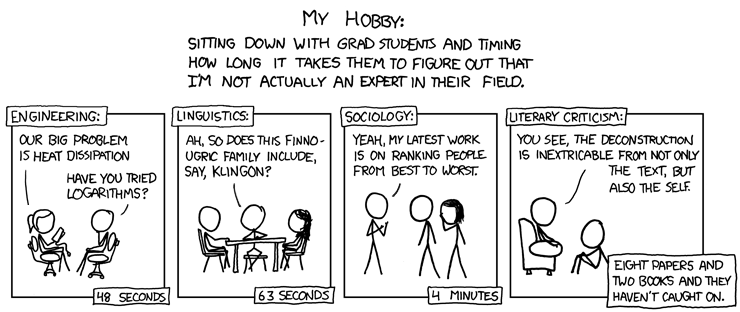
\includegraphics[scale=.5]{comics/451}
\end{center}

\subsubsection{Betriebswirtschaftslehre}

Die Betriebswirtschaftlehre (BWL) ist eine Disziplin der
Wirtschaftswissenschaften, die sich mit den wirtschaftlichen Entscheidungen in
Betrieben und Unternehmen befasst, vor allem mit Art und Menge der zu
beschaffenden Produktionsmittel, Beschaffung und Verwendung der Finanzmittel,
Einsatz der beschafften Produktionsmittel und Veräußerung der Erzeugnisse und
Leistungen. Beim Ergänzungsfach BWL sind regelhaft die folgenden Module zu
absolvieren, die vom Fachbereich Wirtschaftswissenschaften angeboten werden:

\begin{itemize}\itemsep 0pt
    \item Grundlagen des Rechnungswesens (6 LP)
    \item Kosten- und Leistungsrechnung (3 LP)
    \item Unternehmensführung I (3 LP)
    \item Grundzüge der Finanzwirtschaft
          \begin{itemize}\itemsep 0pt
              \item Investition (6 LP)
              \item Finanziernug (6 LP)
          \end{itemize}
\end{itemize}

Bei Fragen wendet euch an eure Tutoren oder an den FSR
Wirtschaftswissenschaften (\url{http://www.wiwifsr.de}).

\begin{center}

\includegraphics[scale=.675]{comics/512}
\end{center}

\subsubsection{Volkswirtschaftslehre}

Die Volkswirtschaftslehre (VWL) teilt sich in die Wirtschaftstheorie (Mikro-
und Makroökonomie), die Wirtschaftspolitik, die Finanzwissenschaft und die
Wirtschafts- und Dogmengeschichte auf. Dabei versucht die VWL, abgelaufene
wirtschaftliche Vorgänge auf einzel- und gesamtwirtschaftlicher Ebene zu
beschreiben, eine beobachtete wirtschaftliche Lage mittels ökonomischer
Theorien zu erklären, Prognosen über zukünftige wirtschaftliche Vorgänge zu
machen und eine wirtschaftspolitische Beraterfunktion einzunehmen.  Beim
Ergänzungsfach VWL sind regelhaft die folgenden Module zu absolvieren, die vom
Fachbereich Wirtschaftswissenschaften angeboten werden:

\begin{itemize}\itemsep 0pt
    \item Mikro- und Makroökonomische Theorie
        \begin{itemize}\itemsep 0pt
              \item Mikroökonomik (6 LP)
              \item Makroökonomik (6 LP)
        \end{itemize}
    \item Ökonometrie
          \begin{itemize}\itemsep 0pt
              \item Angewandte Ökonometrie I (6 LP)
              \item Angewandte Ökonometrie II (6 LP)
          \end{itemize}
\end{itemize}

Auch hier könnt ihr euch natürlich bei Fragen an die Tutoren oder den FSR
Wirtschaftswissenschaften wenden.

\subsubsection{Philosophie}

Ein nach landläufiger Meinung klassisches Nebenfach für die Mathematik ist die
Philosophie. An der Universität Hamburg wird dieses Nebenfach seit neuem
regelhaft angeboten. Ihr habt dabei die Wahl zwischen einem eher theoretischen
oder einem eher praktischen Zugang zu diesem Nebenfach. Die vorgeschlagenen
Modulkombinationen der theoretischen Variante sind

\begin{itemize}\itemsep 0pt
    \item Einführungsmodul Logik und Argumentationstheorie 
    \item Einführungsmodul Praktische Philosophie: Ethik 
    \item Einführungsmodul Theoretische Philosophie 
    \item Aufbaumodul Theoretische Philosophie 
\end{itemize}

\columnbreak

Für die praktische Variante werden die folgende Module vorgeschlagen.

\begin{itemize}\itemsep 0pt
    \item Einführungsmodul Logik und Argumentationstheorie 
    \item Einführungsmodul Praktische Philosophie: Ethik 
    \item Einführungsmodul Theoretische Philosophie 
    \item Aufbaumodul Praktische Philosophie
\end{itemize}

\subsubsection{Technik}

Die Vorlesungen im Ergänzungsfach Technik werden von der Technischen
Universität Hamburg Harburg (TUHH) angeboten. Die TU liegt in der Nähe der
S-Bahn Harburg-Rathaus, und ihr müsst eine gute halbe Stunde Zeit einplanen, um
vom Geomatikum aus dorthin zu gelangen. Regelhaft sind die folgenden Module zu
absolvieren:

\begin{itemize}\itemsep 0pt
    \item Technische Mechanik 1 (4,5 LP)
    \item Technische Mechanik 2 (4,5 LP)
    \item Grundlagen der Elektrotechnik 1 (7,5 LP)
    \item Grundlagen der Elektrotechnik 2 (7,5 LP)
\end{itemize}

Behandelte Themen der Vorlesungen \emphm{Technische Mechanik 1} und \emphm{2}
sind Starrkörperstatik, Elastostatik, Fluidstatik, Kinematik und Kinetik.
\emphm{Grundlagen der Elektrotechnik 1} behandelt Gleichstrom, während der
zweite Teil sich der Wechselstromlehre widmet. Die theoretische Grundlage
dieser beiden technischen Bereiche sowie die Beschreibung ihrer
Gesetzmäßigkeiten sind eng mit verschiedenen Disziplinen der Mathematik
verknüpft. Bei Fragen könnt ihr euch an den FSR Maschinenbau
(\url{www.tu-harburg.de/exp/fsrm}) für Mechanik, den FSR Elektrotechnik
(\url{www.fsr-etit.de}) oder an die Tutoren wenden.

\begin{center}
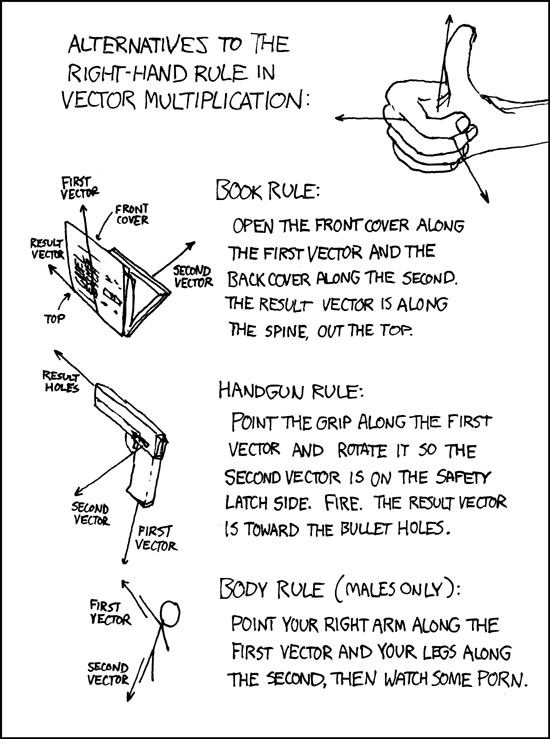
\includegraphics[scale=.66]{comics/199}
\end{center}
